\subsection{Layers}
\label{sec:layers}
\nancomment{could remove archival size from all sections}
In this section we charaterize layer sizes; file and directory counts in
layers; layer compression ratios; and directory depths in the layers.

%%%%%%%%%%%%%%%%%%%%%%%%%%%%%%%%%%%%%%%%%%%%%%%%%%%%%%%%%%%%%%%%%%%%%

\begin{figure}[!t]
	\centering
	\subfigure[CDF of layer sizes]{\label{fig_layer_size_cdf}
		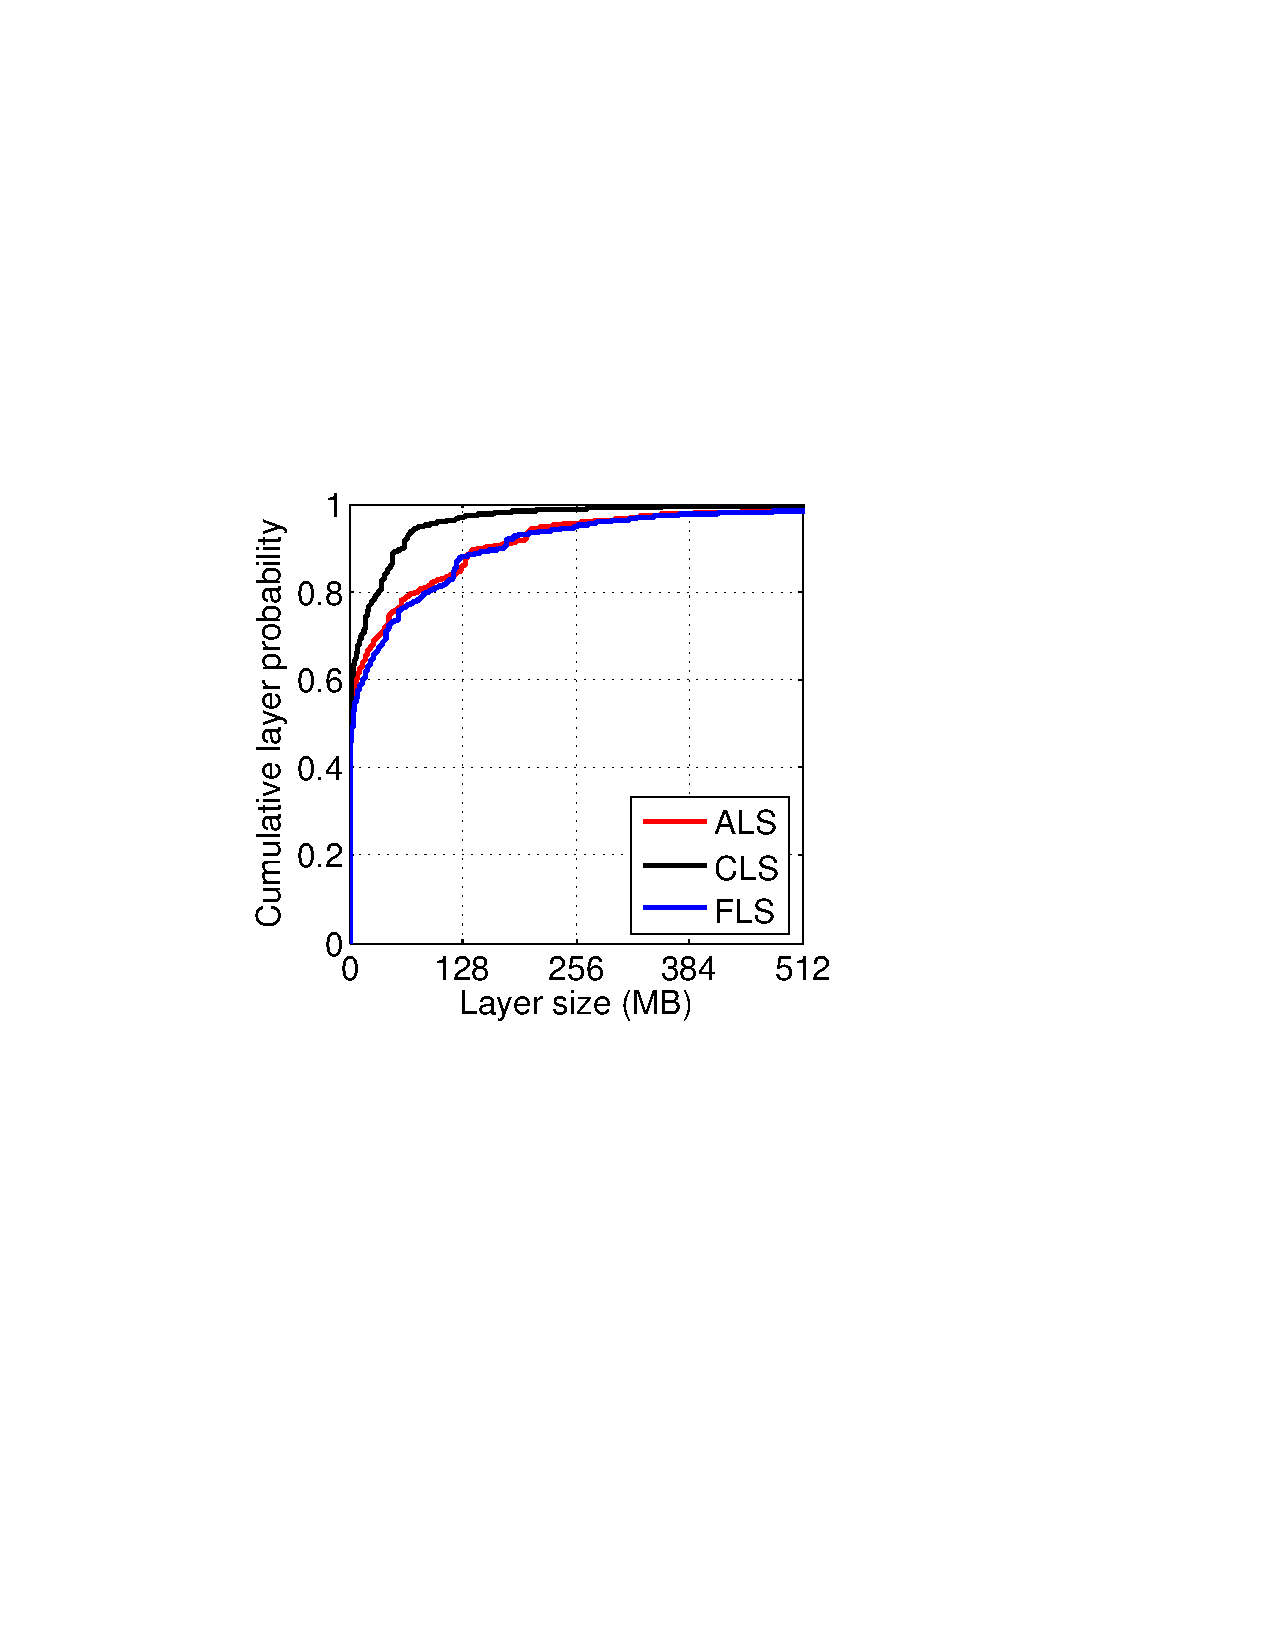
\includegraphics[width=0.234\textwidth]{graphs/layer_size_mb.pdf}
	}
	\subfigure[Histogram of layer sizes]{\label{fig_hist_layer_size}
		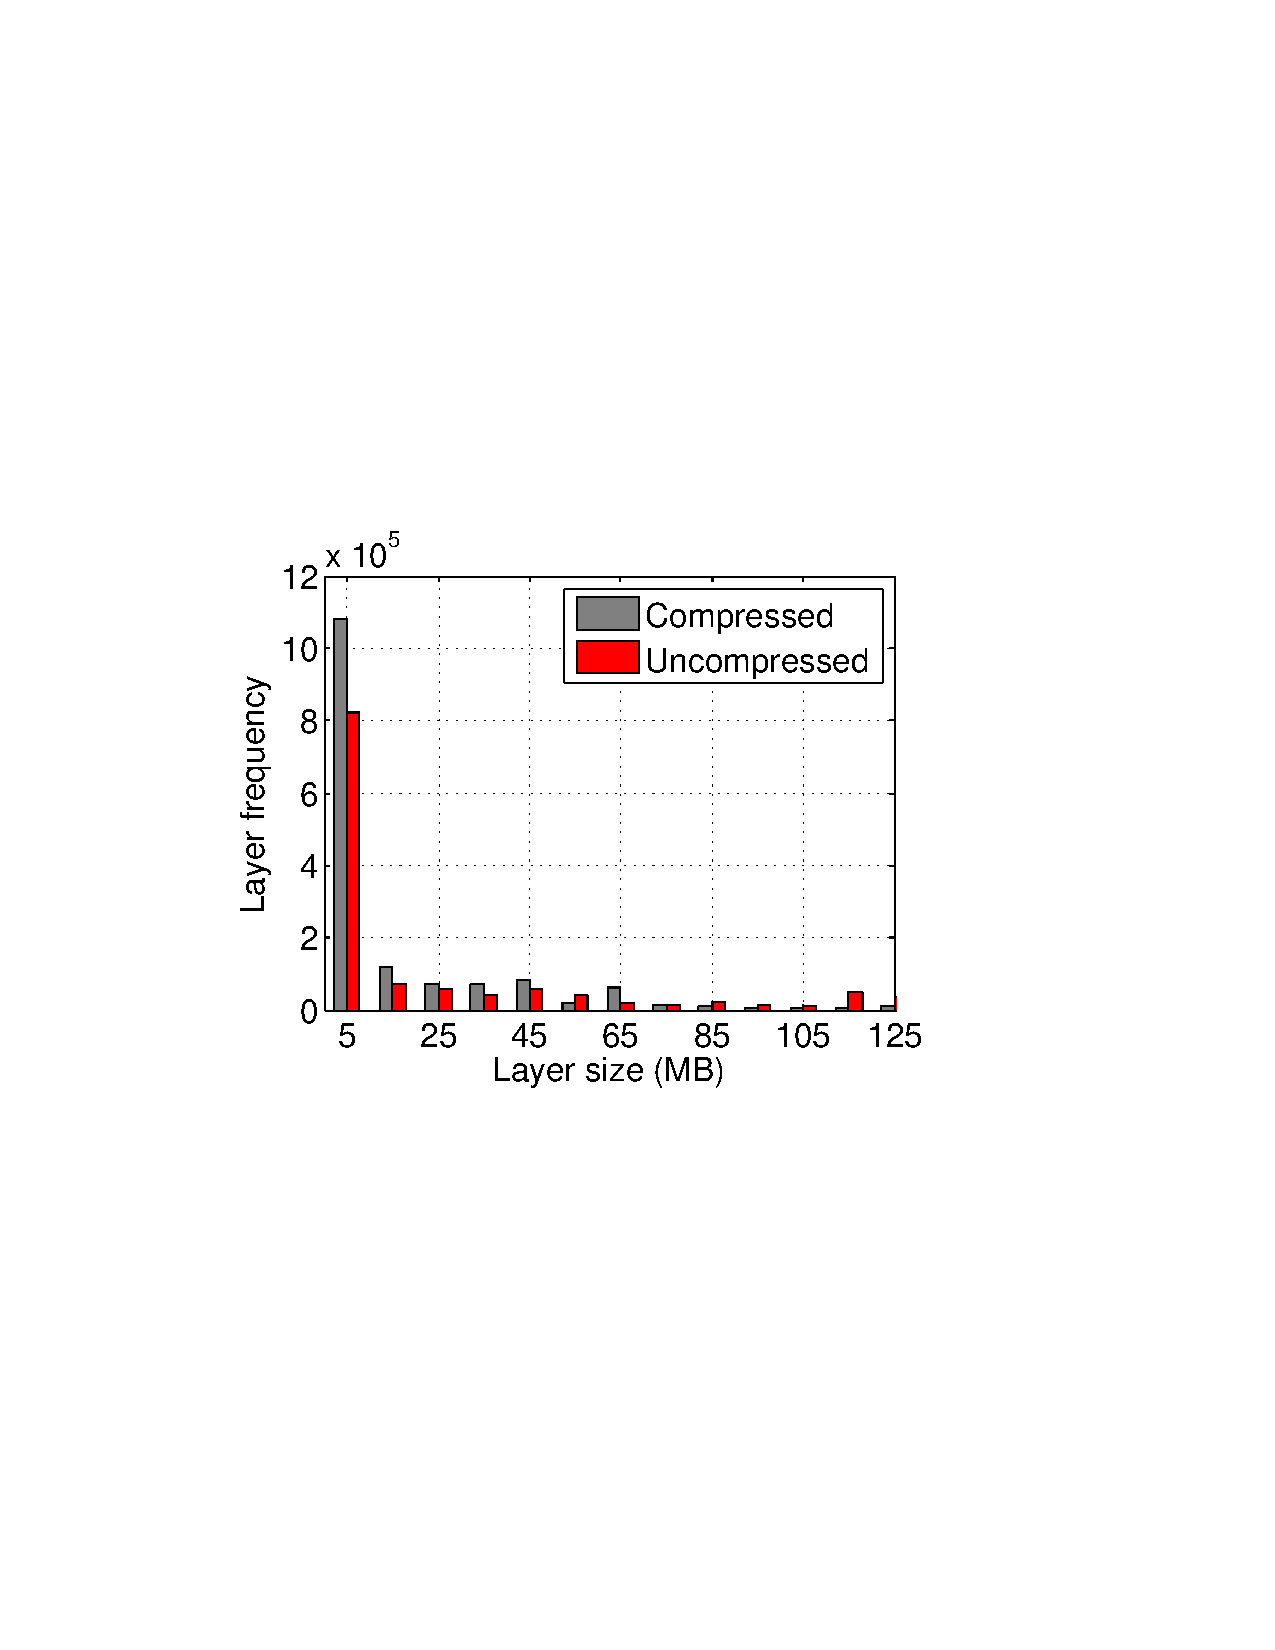
\includegraphics[width=0.213\textwidth]{graphs/hist_layer_size.pdf}
	}
	\caption{Layer size distribution
	\vcomment{Let's use CLS, ALS, and FLS abreviations\nancomment{addressed}}.
	\vcomment{CLS size should go first}.
	\vcomment{We need to use different types of lines (solid, dotted, etc.)
		or markers (round, triangular)}.
	\vcomment{In figure B it is not clear to which bar group corresponds
		  to which layer size. I suggest to try to rotate the graph
		  by 90 grads to fit all layer size labels.\nancomment{aligned label with bar}}
	}
	\label{fig-layer-size}
\end{figure}


\paragraph{Layer sizes}
%
We characterize layer sizes using three different metrics:
%
1)~Compressed Layer Size (CLS)---the format a layer is stored in the registry or
transferred to a client;
%
2)~Archived Layer Size (ALS)---layer in decompressed but archived format;
%
and 3)~Files in Layer Size (FLS)---the sum of containing file sizes.
%
Figure~\ref{fig_layer_size_cdf} shows the CDF of the three metrics.

The ALS and FLS curves are, expectedly, close to each other (within 5\% for
any given layer size) while compressed layers are typically smaller.
%j
90\% of the layers are smaller than 177~MB in uncompressed 
format and smaller than 63~MB in compressed format.
%
Half of the layers are smaller than 4~MB no matter in which format.
%
As we described earlier in \S~\ref{sec:methodology}, we only
analyzed layers smaller than 2~GB in compressed format (this
excluded only XXX\% of the layers).
%
\vcomment{need to adjust Methodology to reflect this.}
%
The largest analyzed uncompresed layer
was of XXX~GB size.
%
Figure~\ref{fig_hist_layer_size} zooms into 0--128~MB range.
%
1,080, 985, and 820 thousands of layers are smaller than 5~MB
in compressed, archived, and unpacked formats, respectively.
%
%90\% of layer can be compressed with less than 63 MB and 77\% of images are
%less than 63 MB even without compression. 

%%%%%%%%%%%%%%%%%%%%%%%%%%%%%%%%%%%%%%%%%%%%%%%%%%%%%%%%%%%%%%%%%%%%%

\begin{figure}[!t]
	\centering
	\subfigure[CDF of compression ratio]{\label{fig_cdf_compression_ratio}
		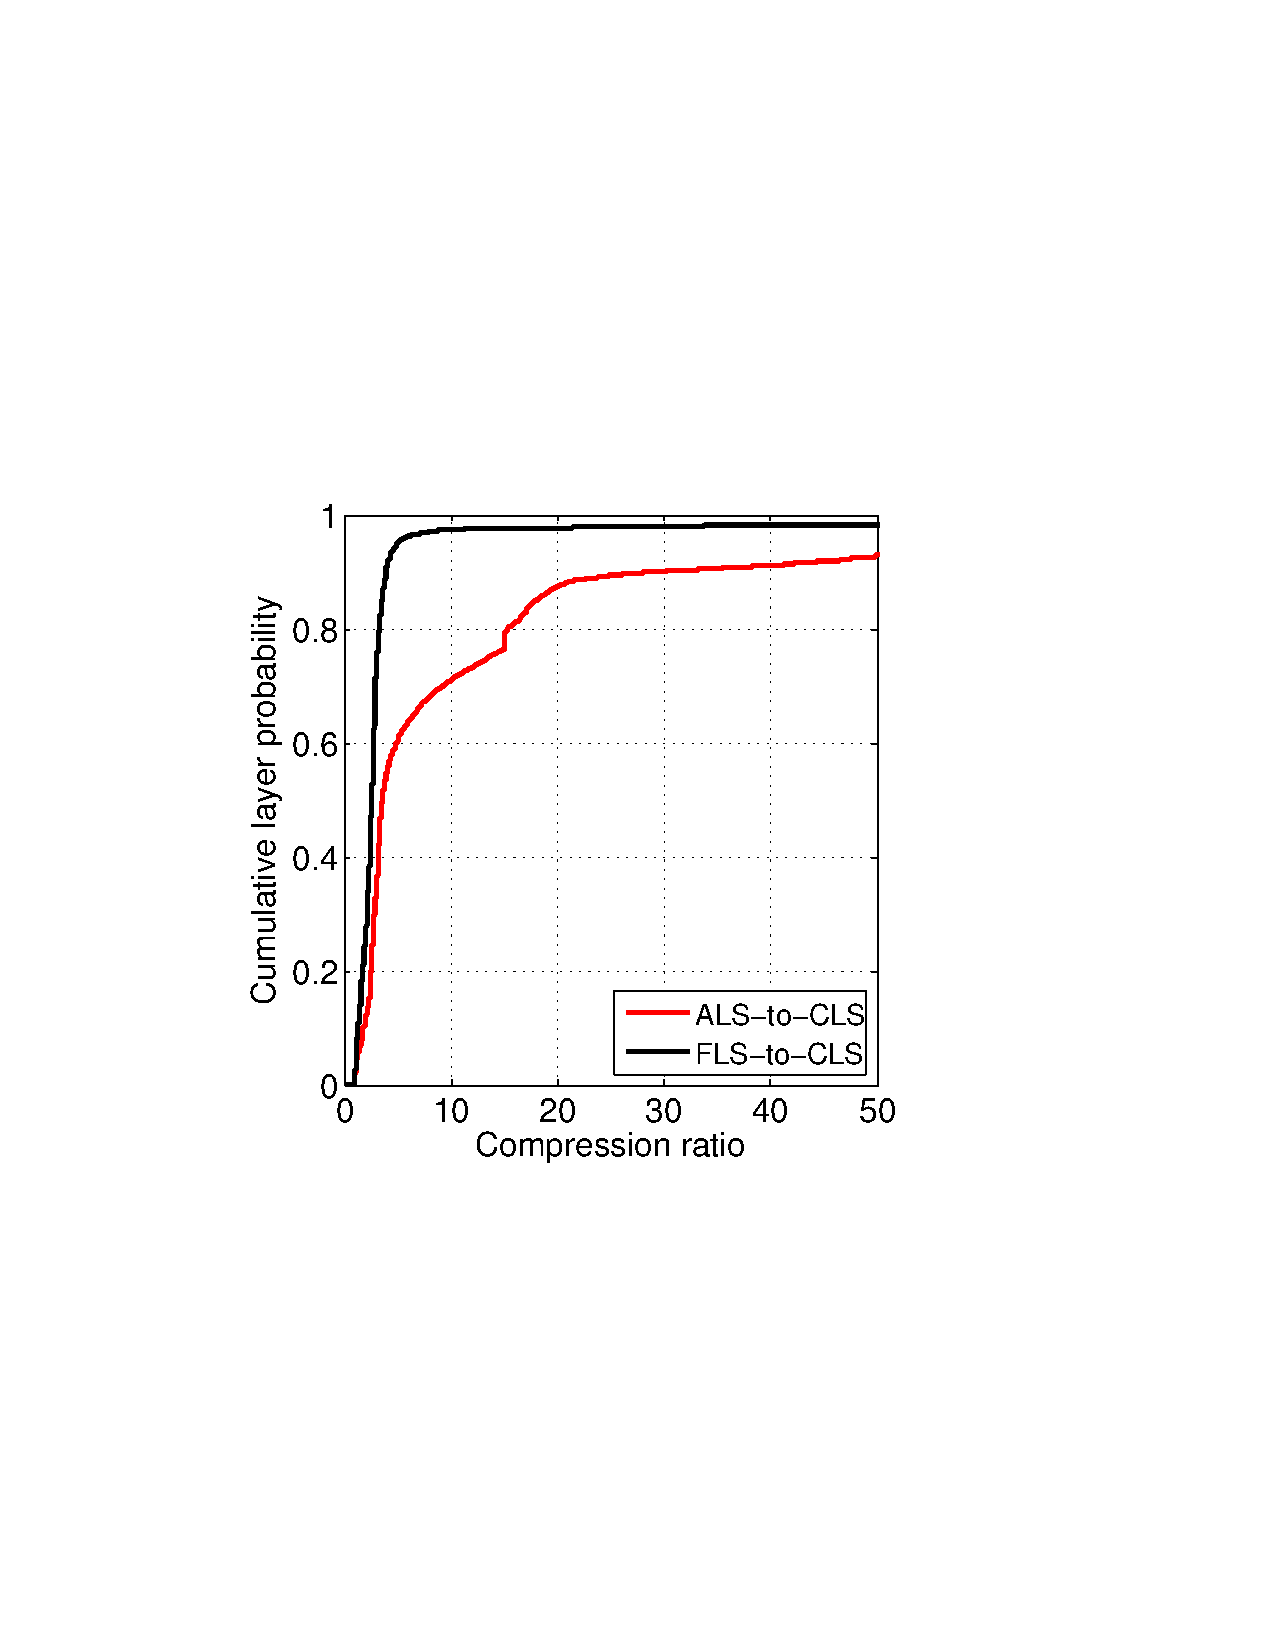
\includegraphics[width=0.23\textwidth]{graphs/cdf_compression_ratio.pdf}
	}
	\subfigure[Histogram of comp. ratios]{\label{fig_his_compression_ratio}
		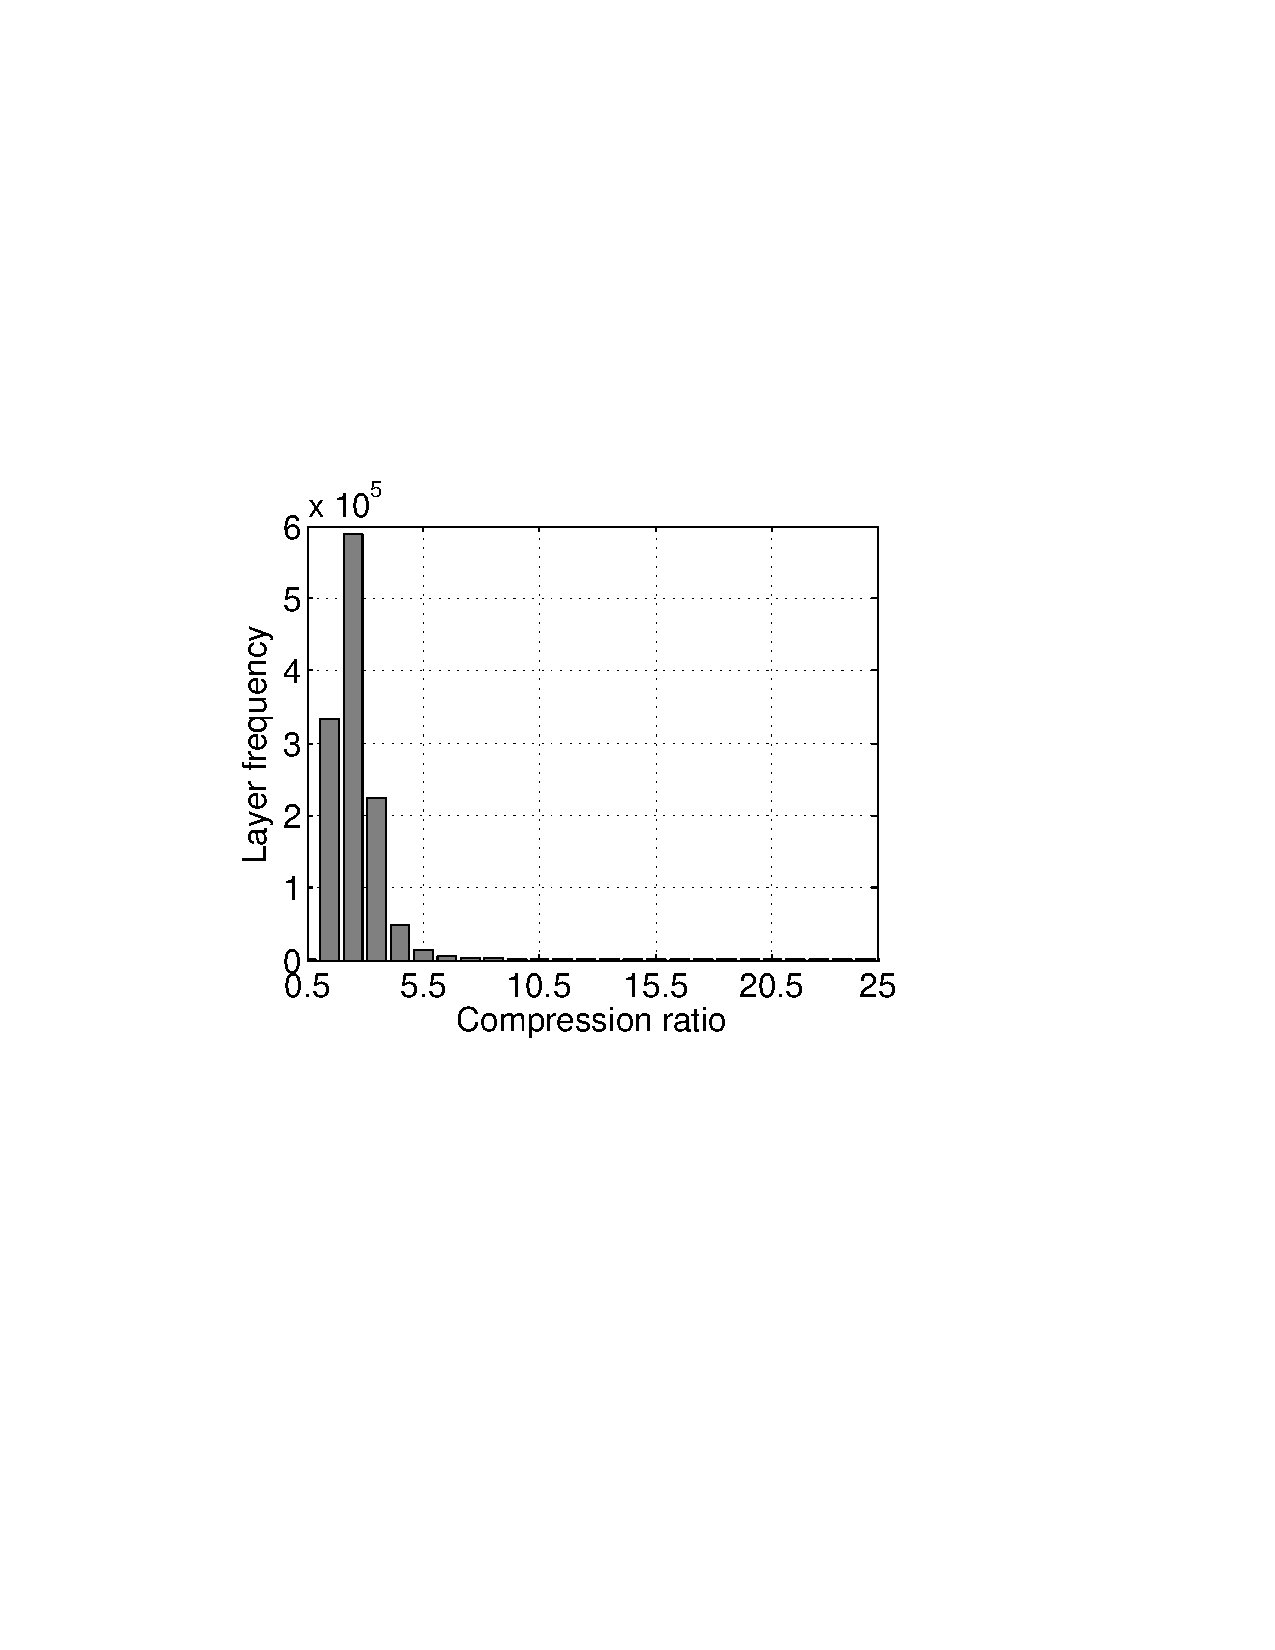
\includegraphics[width=0.223\textwidth]{graphs/his_compression_ratio.pdf}
	}
	\caption{Layer compression ratio distribution
	%\vcomment{Different colors are used in figure (a) and (b) FLS/CLS\nancomment{will address later}}
	}
	\label{fig-compression-ratio}
\end{figure}


\paragraph{Layer compression ratios}
%
We calculated two compression ratios: ALS-to-CLS and FLS-to-CLS.
Figure~\ref{fig_cdf_compression_ratio} shows the CDF of the compression ratios.
%
The ALS-to-CLS ratio is generally greater than the FLS-to-CLS ratio
because small files in layers get larger when combined in a tar archive.
%
90\% of layers have a  ALS-to-FLS ratio less than 4 while 90\% of
layers have FLS-to-CLS ratio less than 30.
%
Half of the layers have a compression ratio (both ALS-to-CLS and
FLS-to-CLS) around 3.
%
The maximum FLS-to-CLS is 512,930 and maximum ALS-to-CLS is 1026.
%
Figure~\ref{fig_his_compression_ratio} shows a histogram of layers by
compression ratio.
%
Two peaks in the graph correspond to 587,000 layers that have the FLS-to-CLS ratio of 3
and 331,000 layers that have the ALS-to-CLS ratio of 3.

%%%%%%%%%%%%%%%%%%%%%%%%%%%%%%%%%%%%%%%%%%%%%%%%%%%%%%%%%%%%%%%%%%%%%

\begin{figure}
	\centering
	\begin{minipage}{0.23\textwidth}
		\centering
		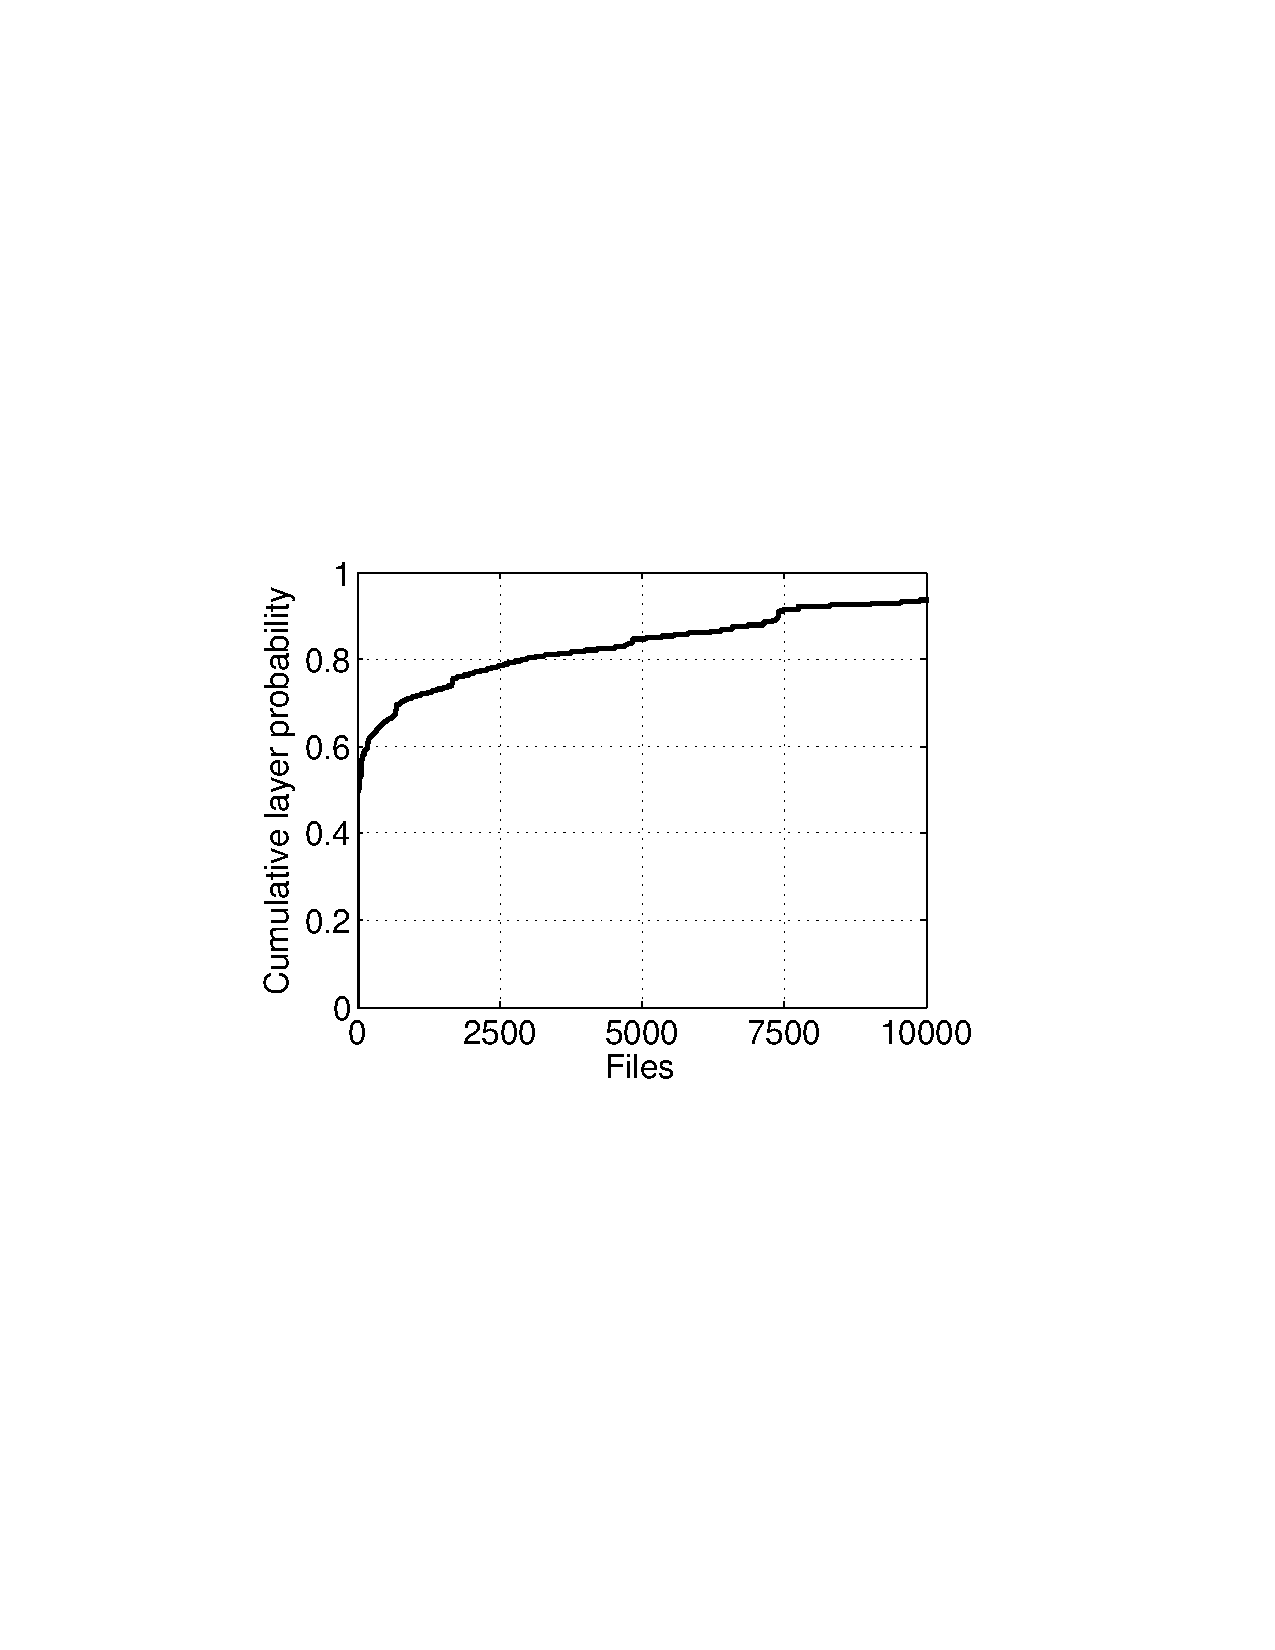
\includegraphics[width=1\textwidth]{graphs/file_cnt.pdf}
		\caption{File count distr.}
		\label{fig_file_cnt}
	\end{minipage}
	\begin{minipage}{0.23\textwidth}
		\centering
		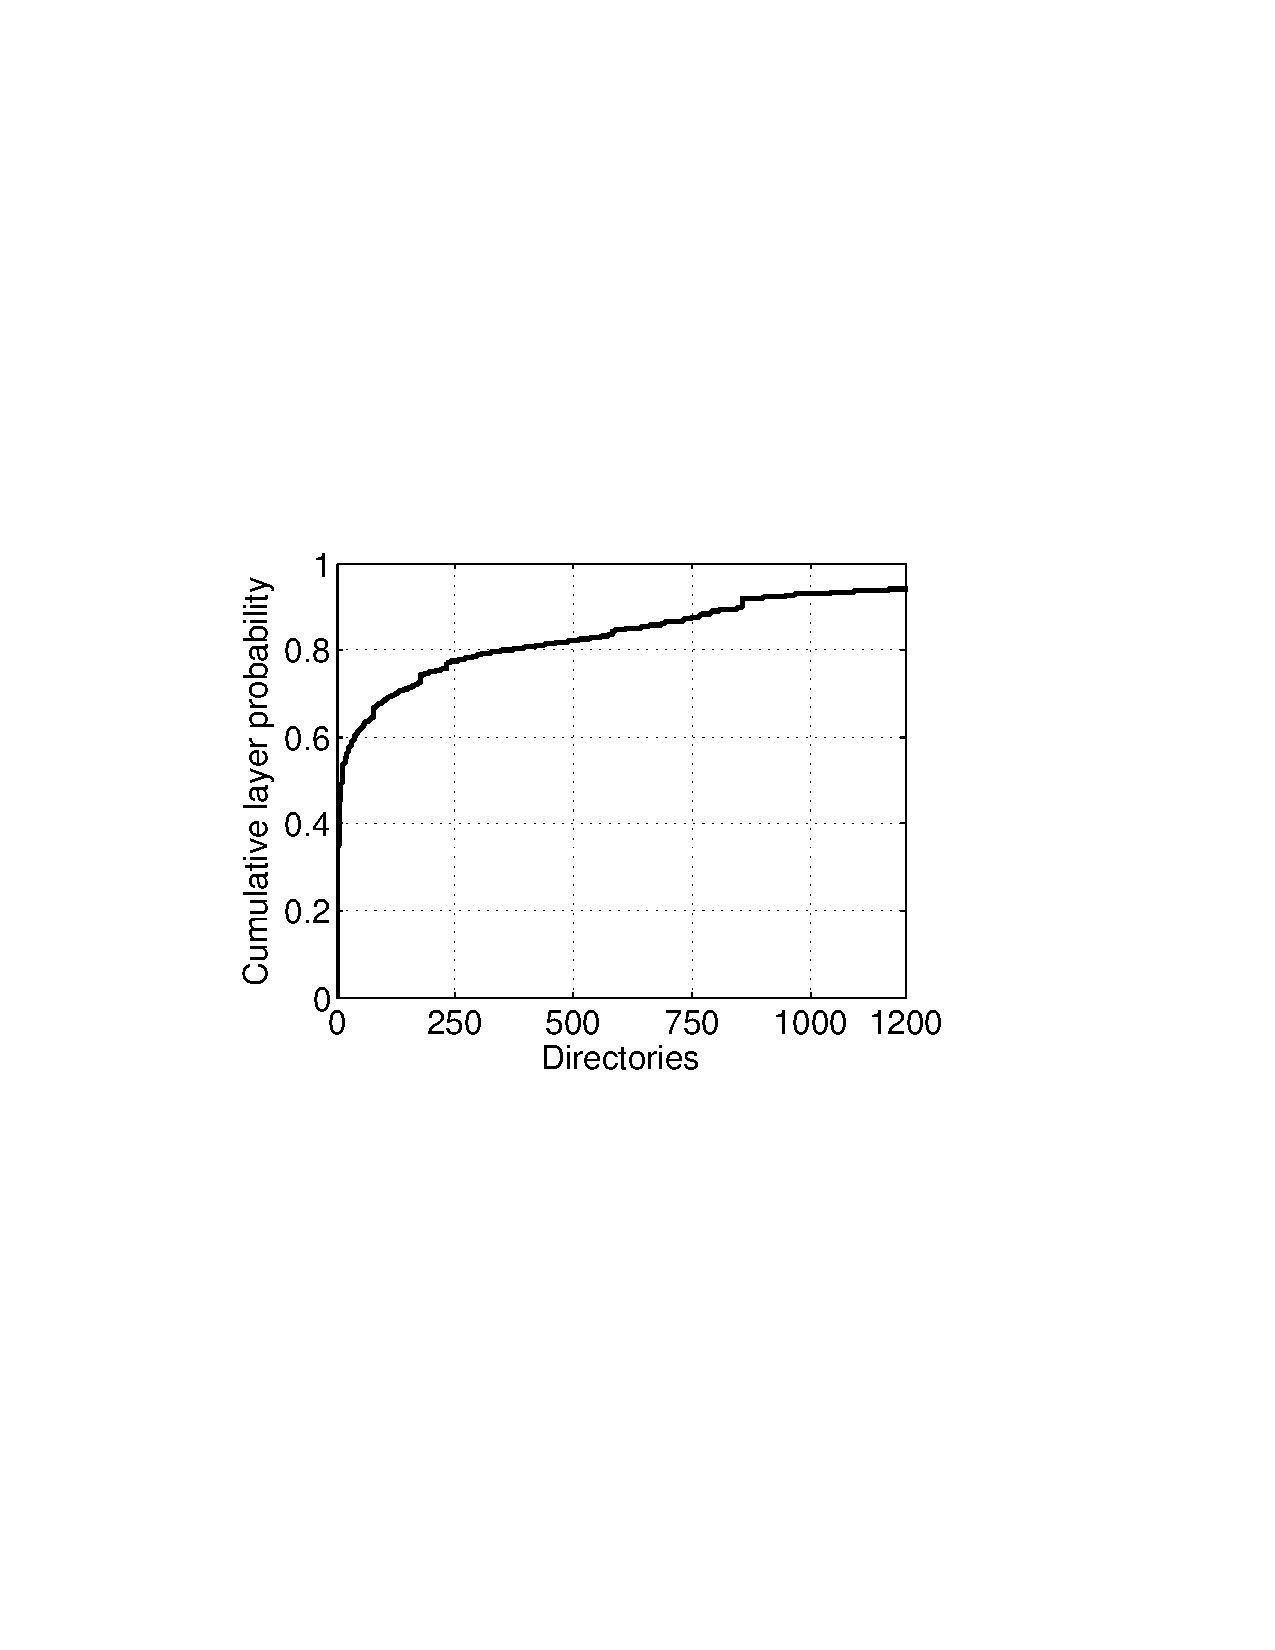
\includegraphics[width=1\textwidth]{graphs/dir_cnt.pdf}
		\caption{Dir. count distr.
		\vcomment{Let's make thise figure subfigures.}
		}
		\label{fig_dir_cnt}
	\end{minipage}%
\end{figure}
%

\paragraph{File and directory counts}

Figure~\ref{fig_file_cnt} and Figure~\ref{fig_dir_cnt} show the CDFs of file
and directory counts for layers.
%
90\% of layers contain less than 7,410 files, while half the of layers have
less than 30 files.
%
XXX\% of the layers have only one file while the largest layer contains 826,196
files.
%
The average is 2,200.
%
The maximum number of directories in a layer is 111,940, the minimum is 1, and
the average is 273.
%
90\% of the layers have less than 826 directories and half of the layers store
less than 11 directories.
%

%%%%%%%%%%%%%%%%%%%%%%%%%%%%%%%%%%%%%%%%%%%%%%%%%%%%%%%%%%%%%%%%%%%%%

\paragraph{Directory depths}

%After extracting and unpacking gzip compressed layer archival files,
We also calculated the maximum directory depth for every layer.
%
Figure~\ref{fig_layer_depth} shows the cumulative layer probability by layer
directory depth.
%
Around 90\% of layers' maximum directory depth is less than 10
and 50\% of layers'  maximum directory depth is less than 4. 
%
Figure~\ref{fig_hist_layer_depth} shows the histogram of layers by
maximum layer directory depth.
%
About 313,000 layers' layer directory depth is 3, which is the peak value in
the figure.
%
%The maximum repeat count is 444 while the median is 4. The average is ~5.

\begin{figure}[!t]
	\centering
	\subfigure[CDF of layers by layer directory depth]{\label{fig_layer_depth}
		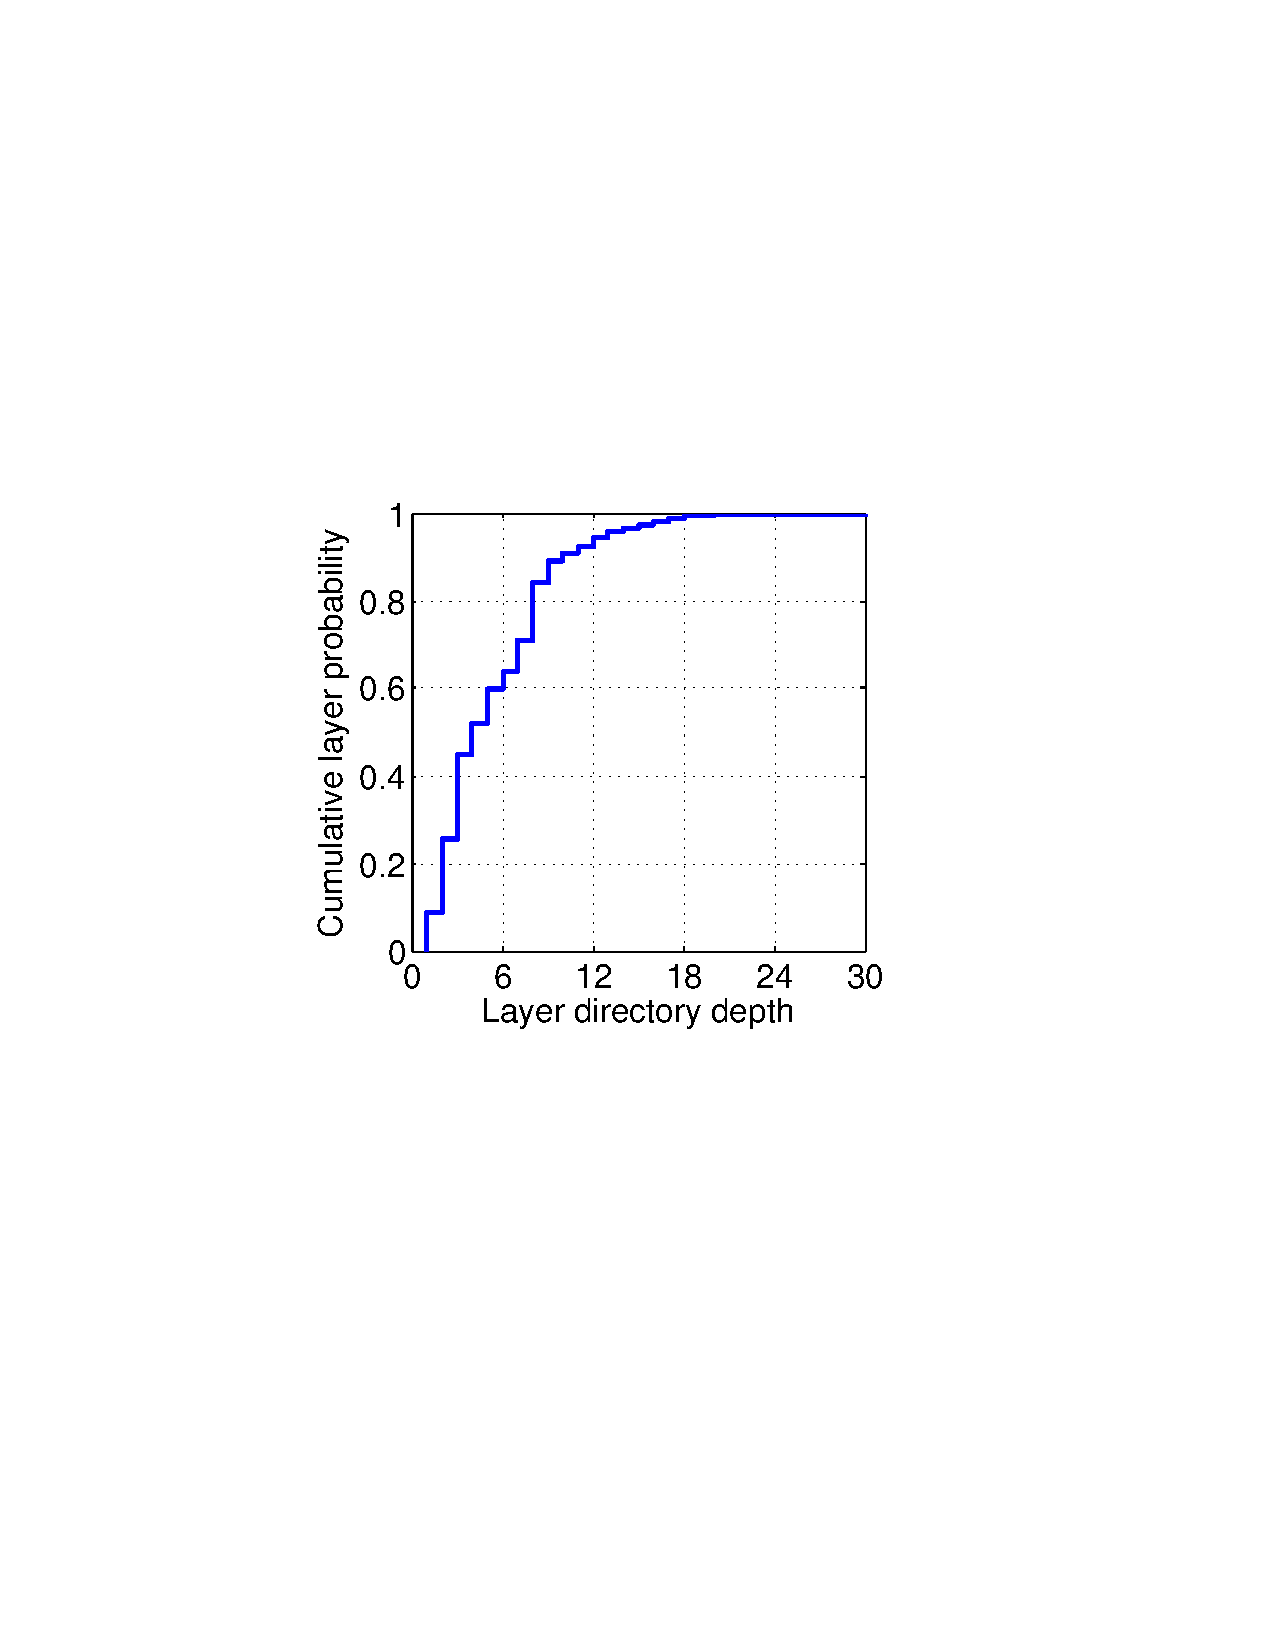
\includegraphics[width=0.23\textwidth]{graphs/layer_depth.pdf}
	}
	\subfigure[Histogram of layers by layer directory depth]{\label{fig_hist_layer_depth}
		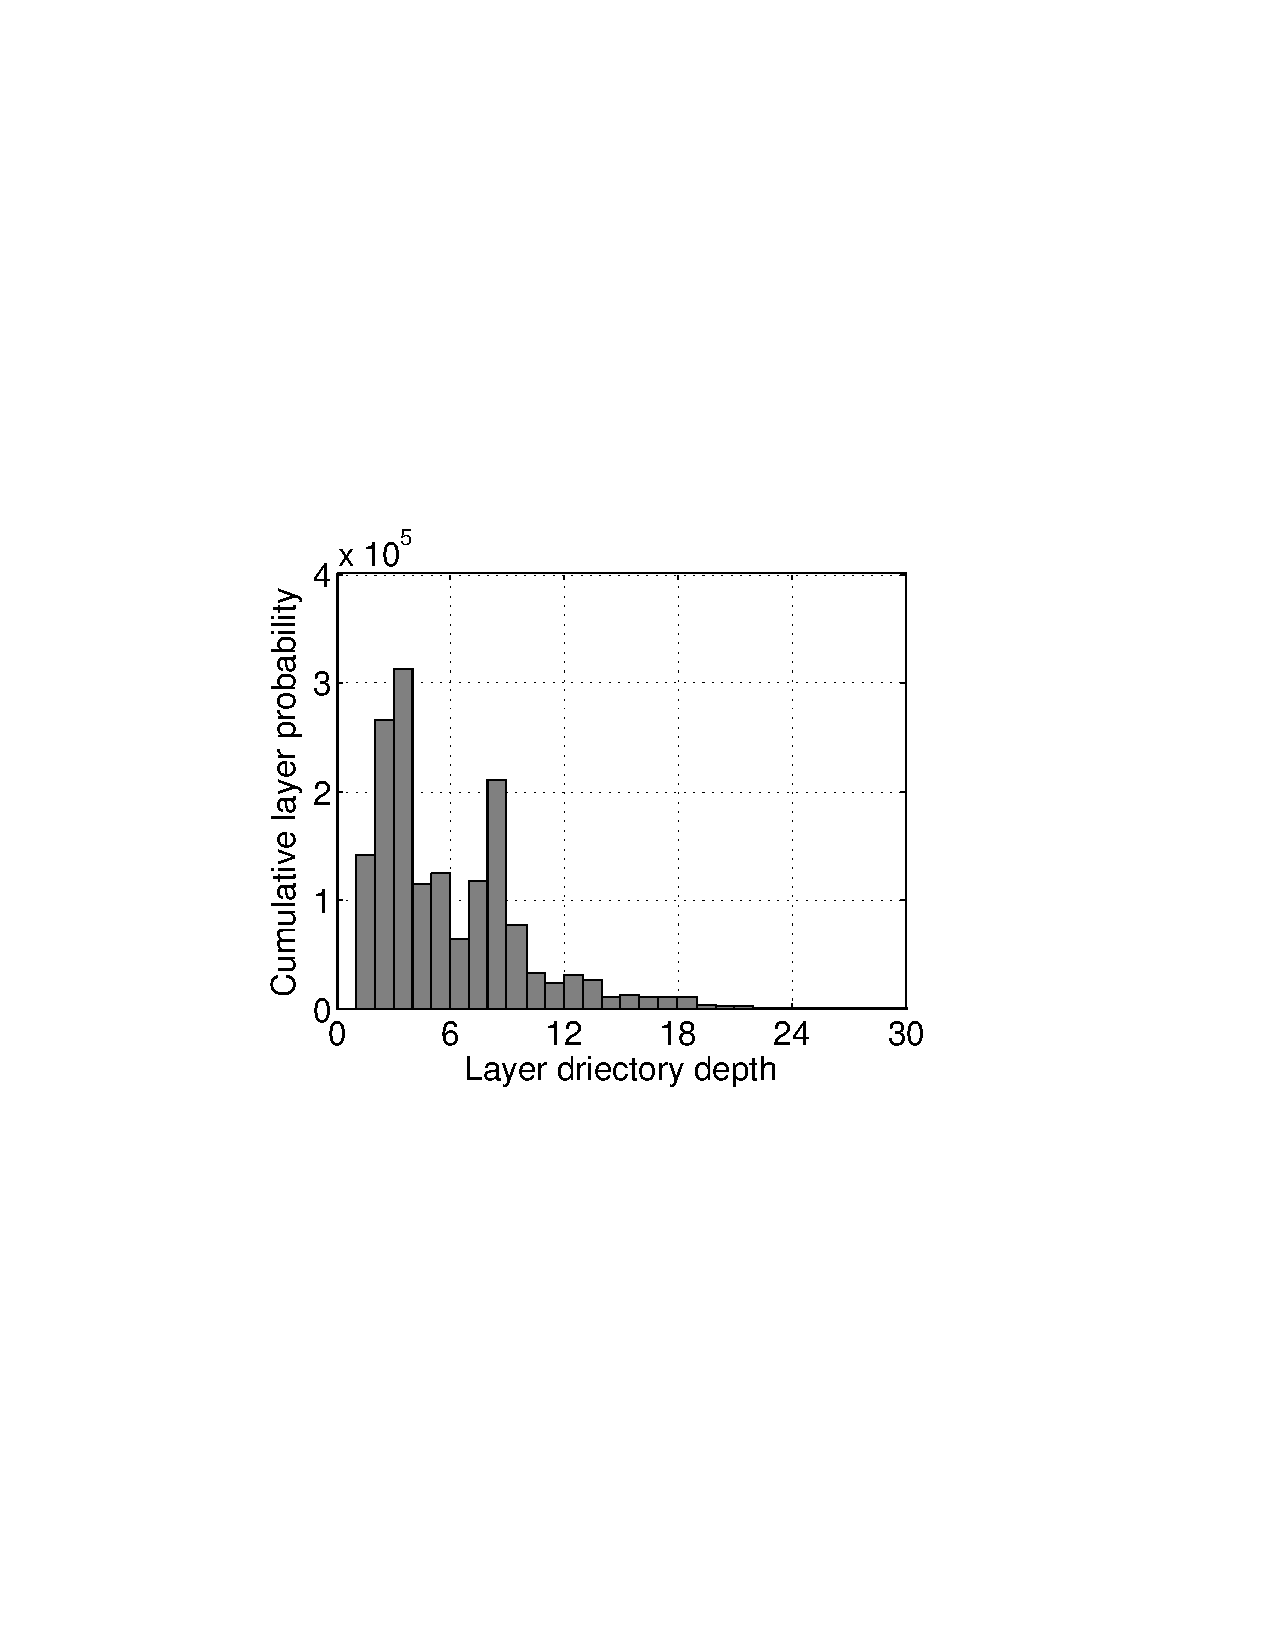
\includegraphics[width=0.22\textwidth]{graphs/hist_layer_depth.pdf}
	}
	\caption{Layer directory depth distribution}
	\label{fig-layer-dir}
\end{figure}
